\section{Apparent Size and Distance}

\answerspace{0.5in}
%\centerline{\epsfxsize 3in\epsfbox{localdistance/calvin-sun.eps}}
%{\centering 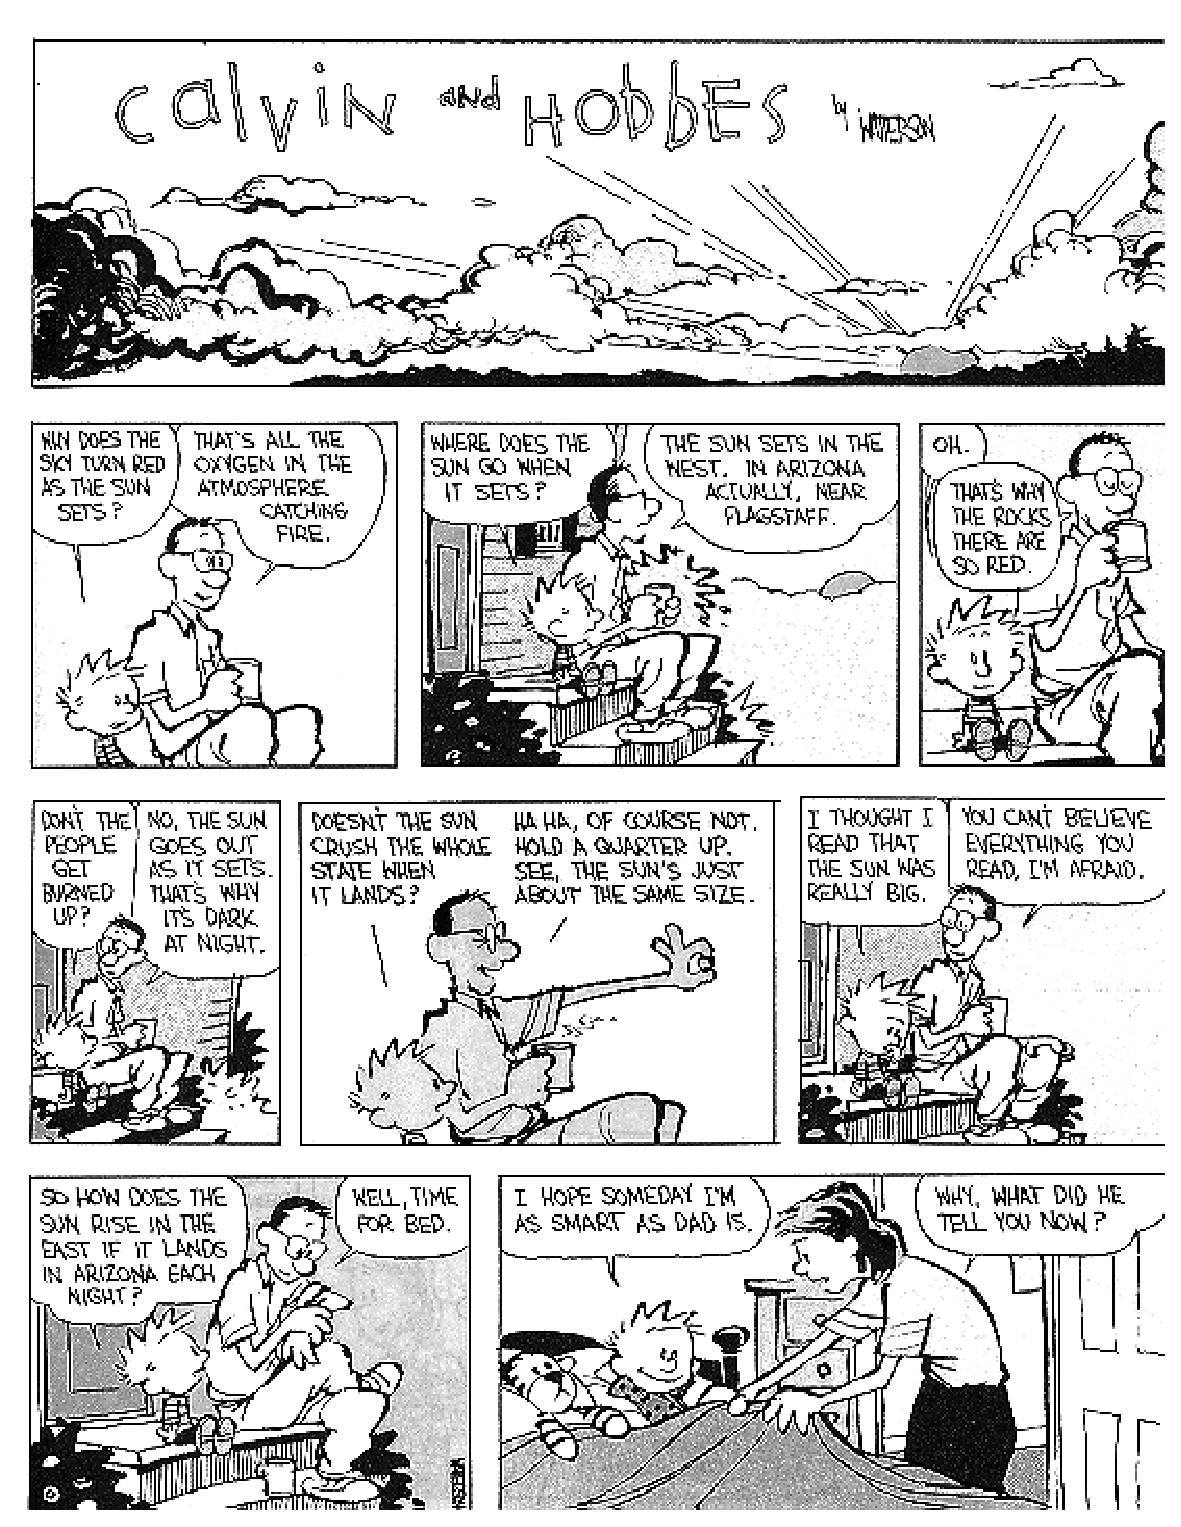
\includegraphics[width=3in]{localdistance/calvin-sun.eps}\par}
\centerline{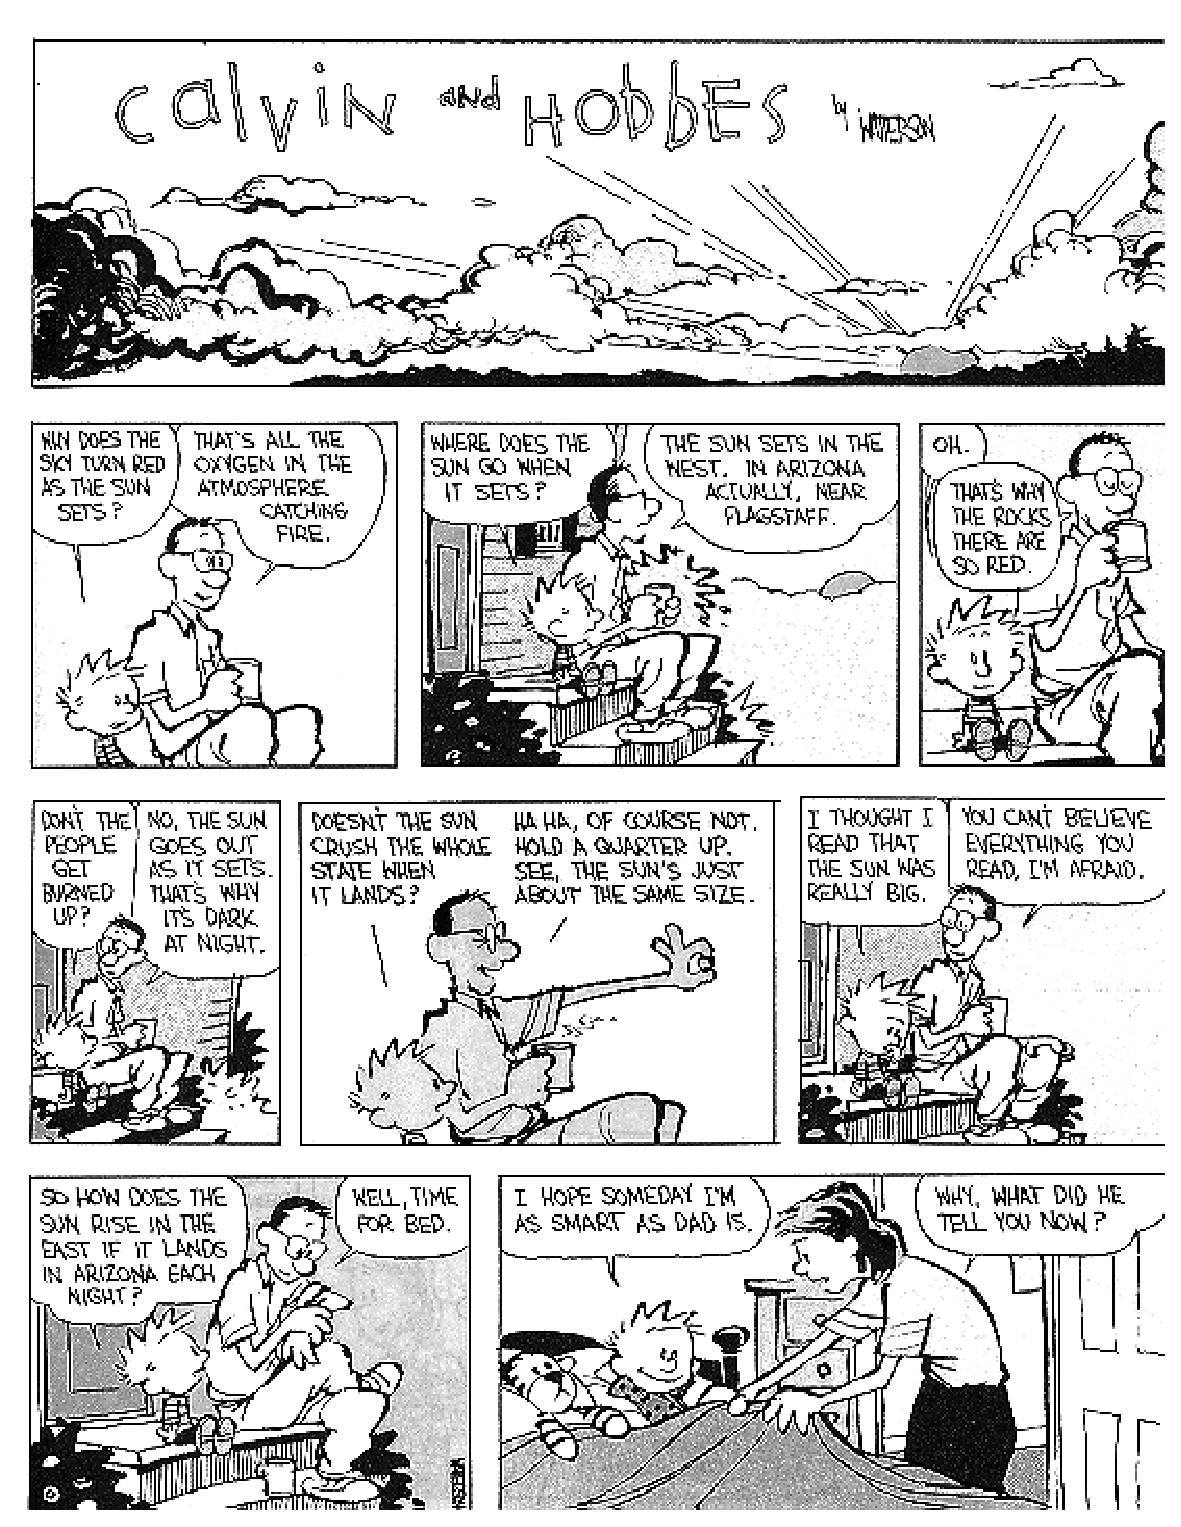
\includegraphics[width=4in]{localdistance/calvin-sun.eps}}
\answerspace{0.5in}

One of the most important things to know about an astronomical
object is its distance from us.  Unfortunately, measuring distances
is often very hard.  There's no one method that works for
finding the distances to all astronomical objects, so 
astronomers have come up with a number of different
methods that work in different circumstances.

One method is based on the simple and obvious observation that a 
faraway object looks smaller than an identical nearby object.
One way to gauge the distance to an object, then, it to measure
its apparent size.  The smaller the apparent size, the greater
the distance.

For instance, suppose you wanted to know the distance to a faraway
galaxy.  Also, suppose that there's a much closer object of the
same apparent size (like the Sun and the quarter Calvin's Dad is holding).
If the two objects have the same apparent size, then the nearby one
can just block the view of the faraway one, like this:

\pagebreak[3]

%\centerline{\epsfxsize 6in\epsfbox{localdistance/localdistance1.eps}}
\centerline{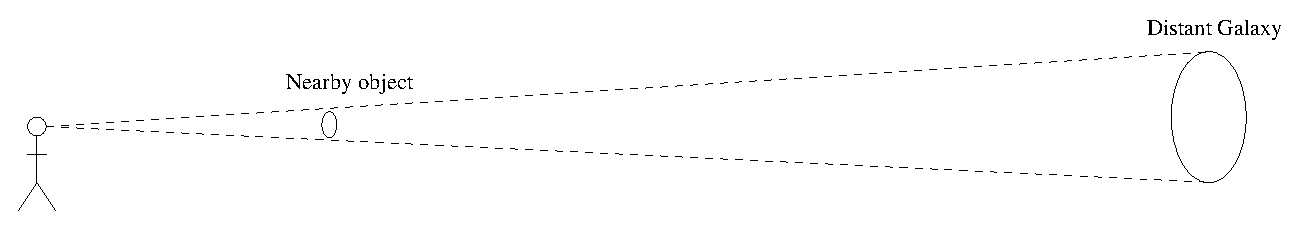
\includegraphics[width=6in]{localdistance/localdistance1.eps}}

Let's give some names to the sizes and distances in this picture:
\begin{itemize}
\item $s_1$ is the size (diameter) of the nearby object.
\item $d_1$ is the distance from the observer to the nearby object.
\item $s_2$ is the size (diameter) of the distant galaxy.
\item $d_2$ is the distance from the observer to the distant galaxy.
\end{itemize}

Indicate these four distances on the diagram above.  Then write down 
an equation giving the mathematical relationship between these
quantities.  (Hints: You might want to think in terms of 
proportions and ratios.  You might possibly want to think back to 
what you learned about similar triangles in geometry class all those years ago.
If you're stuck on this --- or anything else --- ask me.)

\vskip 1in

If we can somehow manage to determine the size and distance of
the nearby object, and the size of the faraway galaxy, we can 
use this relationship to find the galaxy's distance.

To see how this works in practice, you're going to use this
technique to measure the distance to a nearby building on campus.

\begin{enumerate}

\item You have a sheet of transparent plastic with lines of different
thicknesses marked on them.  Take the sheet outside and find a place
where you have a clear view of one of the windows of a nearby 
building (Gray Court and the Modlin Center are the best choices).  Bring
a length of string and a meter stick with you.

\item One partner should hold up the plastic sheet with the lines
oriented horizontally and adjust the sheet so that one of the lines just
blocks the window in the distant
building (that is, so that the apparent thickness
of the line is the same as the apparent height of the window).
The other partner should measure the distance from the person's eye to
the line.  (I suggest you stretch the string between the eye and
the plastic sheet, then measure the length of the string.)
Write down those values here.  Also, write down the thickness of the
line that you used.

{\bf Note:} Whenever you write down a measurement,
you must also write down its units.

\vskip 1in

\item To determine the distance to the other building, you'll need one more bit
of information: the actual size of the window.  We're going to make
an assumption (which may not be correct) that the windows in the other
building
are the same size as the windows in our classroom.  Go back
to the classroom, measure the height of the window, and record it here.

\vskip 1in

\item Using the relationship between $s_1,d_1,s_2,d_2$, together
with the values you just recorded, determine the distance
from here to the other building:

\vskip 1in

To see how well you did, determine the distance using
the
aerial photograph from Google maps
that I'll hand out. Here's how.

\item The scale bar at the lower left of the photograph
shows the distance on the page that corresponds to 50 meters of
actual distance. Measure the length of this bar, and use the result
to determine how many meters of actual distance correspond to 1 cm
on the page.

\vskip 1in

\item Mark on the page your approximate location when you made the
measurement and the location of the window. Measure the distance between
the two points on the page in centimeters.

\vskip 1in 

\item Use this information to determine the distance from your
observation point to the other building in meters.

\vskip 1in

\end{enumerate}

Are your two determinations of the distance significantly
different?  If so, what do you think the main reasons are?  Which
measurements might have been inaccurate?  What assumptions might
have been incorrect?

\vskip 2in

%\newpage
%
%\begin{center}
%{\bf Lab: Apparent Size and Distance}\\
%{\bf Summary of Key Results}
%\end{center}
%
%\vfil
%
%{\bf NAMES:}
%
%\vfil
%
%Distance from eye to sheet:
%\vfil
%
%Thickness of line on sheet:
%\vfil
%
%Height of window in lab:
%\vfil
%
%Distance to building determined from the above numbers:
%\vfil
%
%Scale of photograph: how many meters corresponds to 1 cm on page?
%\vfil
%
%Distance to building as measured on page:
%\vfil
%
%Distance to building as determined from the above numbers:
%\vfil
%\eject
%
%
%
